\documentclass[portrait,final,a0paper,fontscale=0.290]{baposter}

\usepackage{calc}
\usepackage{graphicx}
\usepackage{amsmath}
\usepackage{amssymb}
\usepackage{relsize}
\usepackage{multirow}
\usepackage{rotating}
\usepackage{bm}
\usepackage{enumitem}
\usepackage{url}
\usepackage{booktabs}

\usepackage{graphicx}
\usepackage{multicol}

%\usepackage{times}
\usepackage{helvet}
%\usepackage{bookman}
%\usepackage{palatino}
\renewcommand*{\familydefault}{\sfdefault}

\newcommand{\captionfont}{\footnotesize}

\graphicspath{{images/}}
%\usetikzlibrary{calc} %TODO del



%%%%%%%%%%%%%%%%%%%%%%%%%%%%%%%%%%%%%%%%%%%%%%%%%%%%%%%%%%%%%%%%%%%%%%%%%%%%%%%%
% Multicol Settings
%%%%%%%%%%%%%%%%%%%%%%%%%%%%%%%%%%%%%%%%%%%%%%%%%%%%%%%%%%%%%%%%%%%%%%%%%%%%%%%%
\setlength{\columnsep}{1.5em}
\setlength{\columnseprule}{0mm}

%%%%%%%%%%%%%%%%%%%%%%%%%%%%%%%%%%%%%%%%%%%%%%%%%%%%%%%%%%%%%%%%%%%%%%%%%%%%%%%%
% Save space in lists. Use this after the opening of the list
%%%%%%%%%%%%%%%%%%%%%%%%%%%%%%%%%%%%%%%%%%%%%%%%%%%%%%%%%%%%%%%%%%%%%%%%%%%%%%%%
\newcommand{\compresslist}{%
\setlength{\itemsep}{1pt}%
\setlength{\parskip}{0pt}%
\setlength{\parsep}{0pt}%
}

%%%%%%%%%%%%%%%%%%%%%%%%%%%%%%%%%%%%%%%%%%%%%%%%%%%%%%%%%%%%%%%%%%%%%%%%%%%%%%
%%% Begin of Document
%%%%%%%%%%%%%%%%%%%%%%%%%%%%%%%%%%%%%%%%%%%%%%%%%%%%%%%%%%%%%%%%%%%%%%%%%%%%%%

\begin{document}

%%%%%%%%%%%%%%%%%%%%%%%%%%%%%%%%%%%%%%%%%%%%%%%%%%%%%%%%%%%%%%%%%%%%%%%%%%%%%%
%%% Here starts the poster
%%%---------------------------------------------------------------------------
%%% Format it to your taste with the options
%%%%%%%%%%%%%%%%%%%%%%%%%%%%%%%%%%%%%%%%%%%%%%%%%%%%%%%%%%%%%%%%%%%%%%%%%%%%%%
% Define some colors

\definecolor{lightgreen}{rgb}{0.2,0.9,0.2}
\definecolor{lightestgreen}{rgb}{0.8,1.0,0.5}
\definecolor{darkgreen}{rgb}{0.2,0.4,0.2}
\definecolor{lightorange}{rgb}{0.9,0.4,0}
\definecolor{lightestorange}{rgb}{1,0.8,0.5}
\definecolor{darkorange}{rgb}{0.2,0.1,0}

%\hyphenation{resolution occlusions}
%%
\begin{poster}%
  % Poster Options
  {
  % Show grid to help with alignment
  grid=false,
  % Column
  columns=4,
  colspacing=1em,
  % Color style
  background=shadetb,
  bgColorOne=lightestgreen!80,
  bgColorTwo=white,
  borderColor=darkgreen,
  headerColorOne=darkgreen,
  headerColorTwo=lightgreen,
  headerFontColor=white,
  boxColorOne=lightestgreen,
  boxColorTwo=lightgreen,
  % Format of textbox
  textborder=faded,
  % Format of text header
  eyecatcher=true,
  headerborder=closed,
  headerheight=0.1\textheight,
%  textfont=\sc, An example of changing the text font
  headershape=roundedright,
  headershade=shadelr,
  headerfont=\Large\bf\textsc, %Sans Serif
  textfont={\setlength{\parindent}{1.5em}},
  boxshade=plain,
  linewidth=2pt
  }
  % Eye Catcher
  {
      
\includegraphics[scale=0.5]{logo_irisa_dyliss.png}
  }
  % Title
  {\bf\textsc{POGG and nitrification cycle modelization}\vspace{0.5em}}
  % Authors
  {\textsc{Thibault Etienne}}
  % University logo
  {
    
\includegraphics[scale=0.5]{logo_UR1_UEB.png}
  }

%%%%%%%%%%%%%%%%%%%%%%%%%%%%%%%%%%%%%%%%%%%%%%%%%%%%%%%%%%%%%%%%%%%%%%%%%%%%%%
%%% Now define the boxes that make up the poster
%%%---------------------------------------------------------------------------
%%% Each box has a name and can be placed absolutely or relatively.
%%% The only inconvenience is that you can only specify a relative position 
%%% towards an already declared box. So if you have a box attached to the 
%%% bottom, one to the top and a third one which should be in between, you 
%%% have to specify the top and bottom boxes before you specify the middle 
%%% box.
%%%%%%%%%%%%%%%%%%%%%%%%%%%%%%%%%%%%%%%%%%%%%%%%%%%%%%%%%%%%%%%%%%%%%%%%%%%%%%



%%%%%%%%%%%%%%%%%%%%%%%%%%%%%%%%%%%%%%%%%%%%%%%%%%%%%%%%%%%%%%%%%%%%%%%%%%%%%%
  \headerbox{Introduction}{name=introduction,column=0,span=1,row=0}{
%%%%%%%%%%%%%%%%%%%%%%%%%%%%%%%%%%%%%%%%%%%%%%%%%%%%%%%%%%%%%%%%%%%%%%%%%%%%%%
    Currently, most of biological modelizations use a trait-based model; but that need a lot of knowledges about modelized system.\\
    \vspace{7pt}\\
    \textsc{Probabilities On Genetic Graph} (POGG) is another model, designed for patterns finding and metabolic network modelizing, based on measurement of studied variables~\cite{JBourdon2011}.\\
    \vspace{7pt}\\
    Here, POGG is used for study\\the Nitrification process\\
    of Nitrogen cycle.
 }


%%%%%%%%%%%%%%%%%%%%%%%%%%%%%%%%%%%%%%%%%%%%%%%%%%%%%%%%%%%%%%%%%%%%%%%%%%%%%%
  \headerbox{Nitrogen cycle and Nitrification}{name=biology,column=1,span=3,row=0}{
  %%%%%%%%%%%%%%%%%%%%%%%%%%%%%%%%%%%%%%%%%%%%%%%%%%%%%%%%%%%%%%%%%%%%%%%%%%%%%%
    \begin{minipage}{\linewidth}
        \begin{minipage}{0.65\linewidth}
            \textsc{Figure 1:} Nitrogen cycle, interesting in many ways\\(economic, ecologic,...)
            \\
            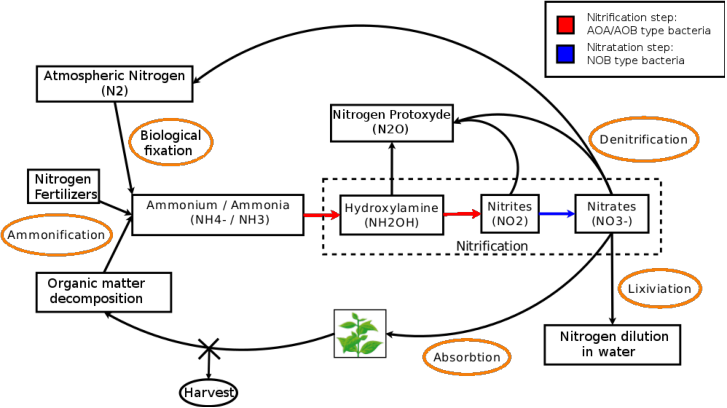
\includegraphics[width=0.9\linewidth]{biology_natrium_cycle_eng}
        \end{minipage}
        \begin{minipage}{0.35\linewidth}
            This work keep focus\\on Nitrification (Fig.1),\\where Ammonia, Nitrite\\and Nitrateare the main\\studied elements.\\
            \vspace{4pt}\\
            See Fig.2 for their\\exact measures.
        \end{minipage}
    \end{minipage}
    \vspace{7.5pt}\\
  }


%%%%%%%%%%%%%%%%%%%%%%%%%%%%%%%%%%%%%%%%%%%%%%%%%%%%%%%%%%%%%%%%%%%%%%%%%%%%%%
  \headerbox{POGG and modelization process}{name=pogg,row=1,column=0,span=4,below=introduction}{
%%%%%%%%%%%%%%%%%%%%%%%%%%%%%%%%%%%%%%%%%%%%%%%%%%%%%%%%%%%%%%%%%%%%%%%%%%%%%%
    \begin{minipage}{\linewidth}
        \begin{minipage}{0.3\linewidth}
            POGG use Markov chains, probabilities\\matrix and cost matrix, 
            which are deduced from collected data (concentration variation, Fig.2) or general knowledge (Nitrification process, Fig.1).\\
            \vspace{8pt}\\
            These data are used in a learning process, which is is the model construction, through formatting and optimization of external data.\\
            \vspace{8pt}\\
            After few steps of data treatments, \textit{unique transition matrix} is generated; \\
            Learning step is finished, modelization is the next one.
        \end{minipage}
        \begin{minipage}{0.7\linewidth}
            \begin{center}
                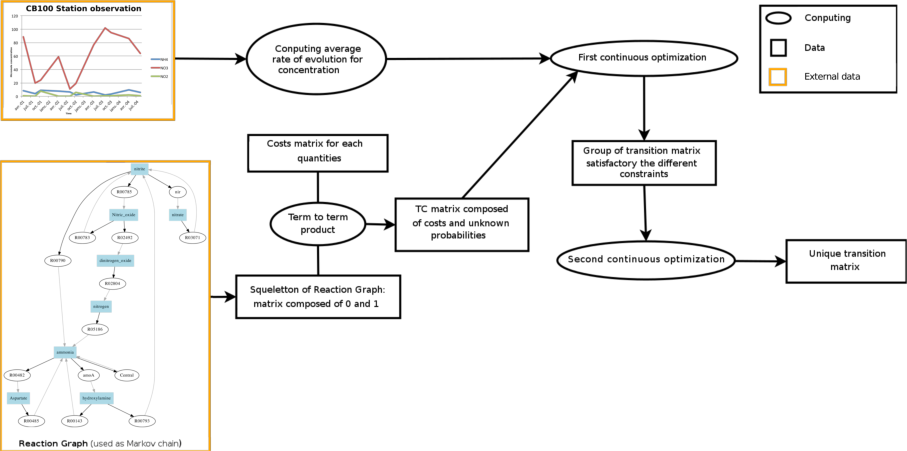
\includegraphics[width=0.90\linewidth]{pogg_process}
                \vspace{2pt}\\
                \textsc{Figure 2:} POGG learning process, from collected to generated data
            \end{center}
        \end{minipage}
        \vspace{2pt}\\
    \end{minipage}
  }


%%%%%%%%%%%%%%%%%%%%%%%%%%%%%%%%%%%%%%%%%%%%%%%%%%%%%%%%%%%%%%%%%%%%%%%%%%%%%%
\headerbox{Modelization results}{name=results,row=2,column=0,span=3,below=pogg}{          %
%%%%%%%%%%%%%%%%%%%%%%%%%%%%%%%%%%%%%%%%%%%%%%%%%%%%%%%%%%%%%%%%%%%%%%%%%%%%%%
    \begin{center}
        \textsc{Figure 3:} season models and final simulation over 3 estimated years
        \vspace{4pt}\\
        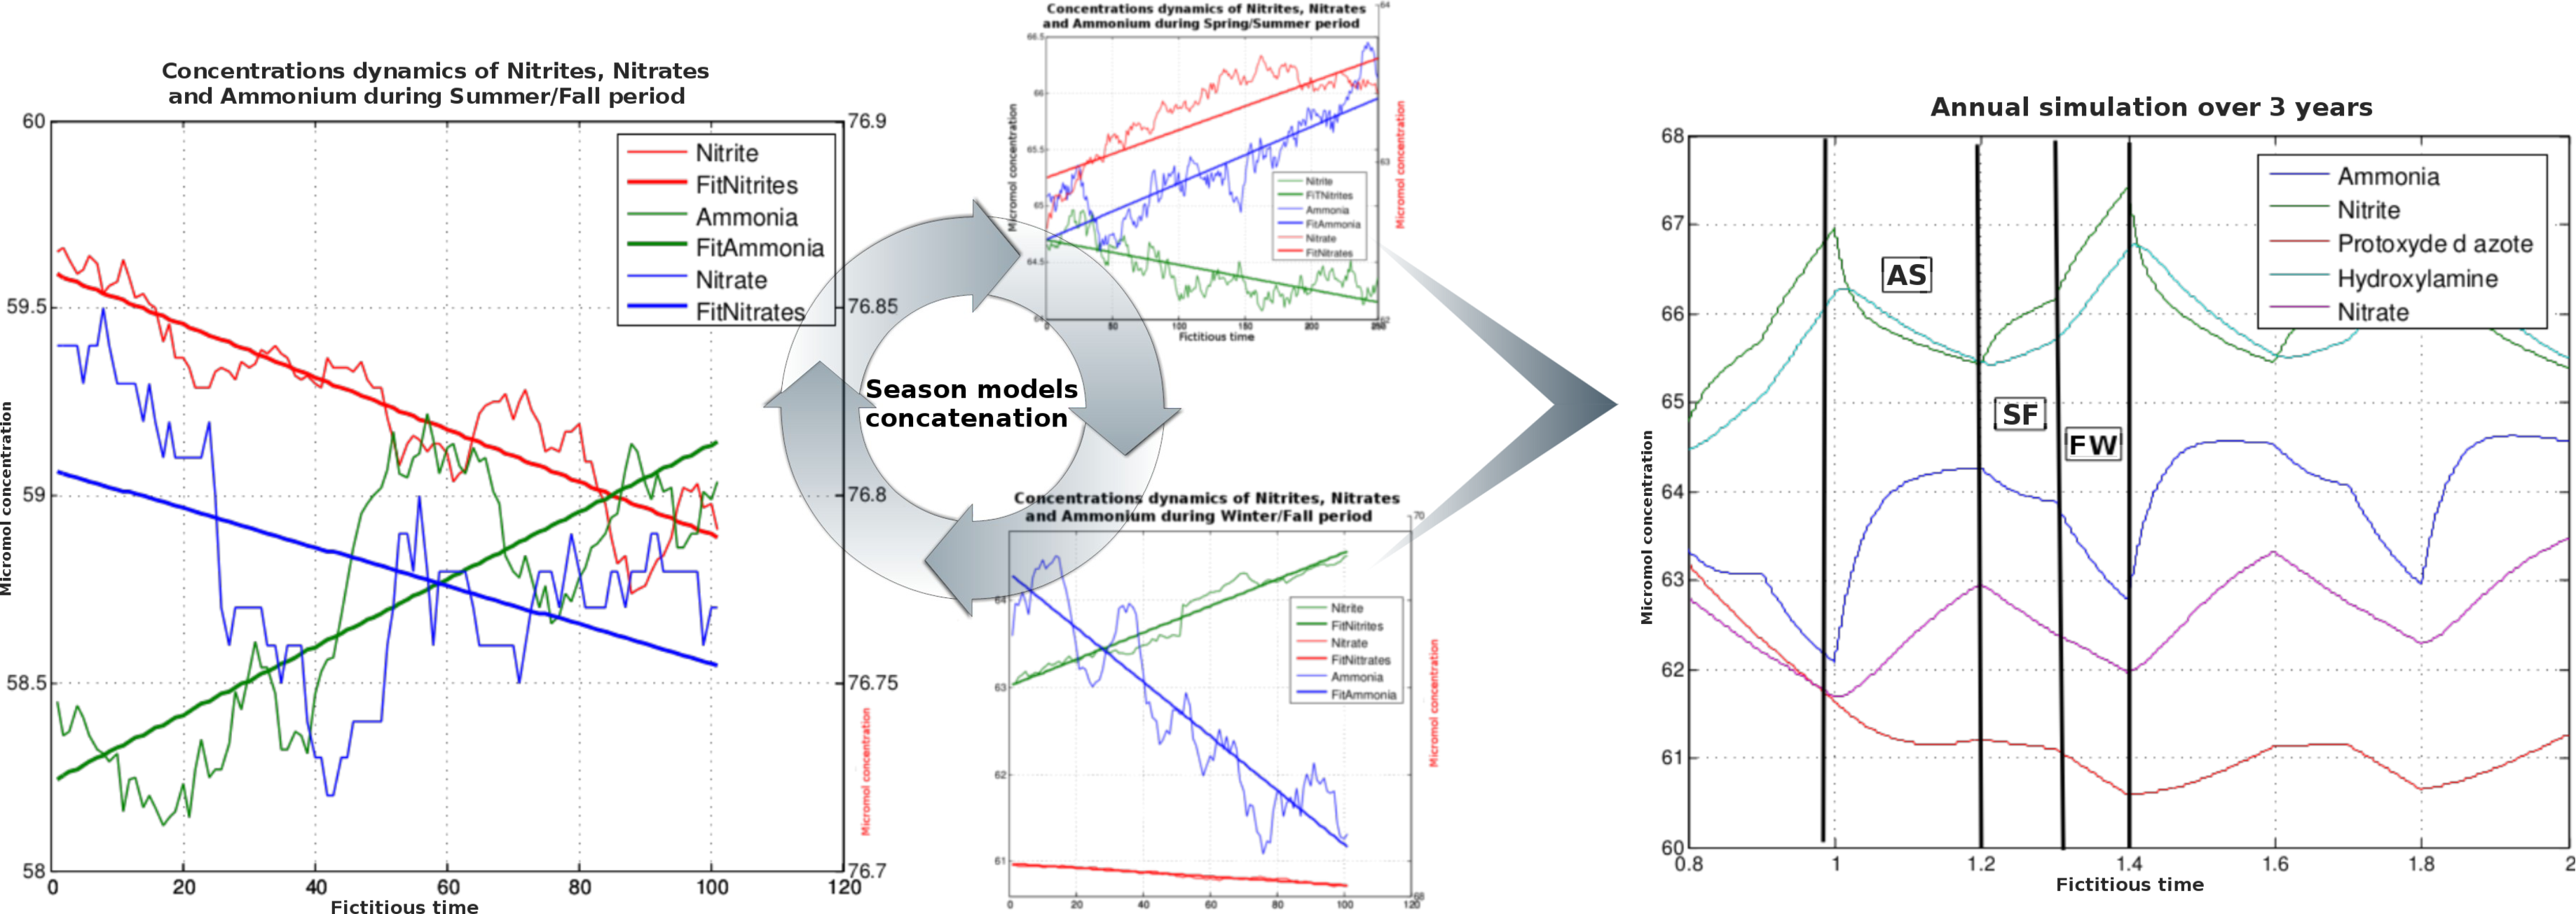
\includegraphics[width=0.85\linewidth]{results_final_season3}
    \end{center}
    \begin{minipage}{\linewidth}
      \begin{minipage}{0.05\linewidth}
      \end{minipage}\hfill
      \begin{minipage}{0.45\linewidth}
              Each seasons have its own model (Fig.3);\\
              for modelize an entire year,\\season models are concatened.
      \end{minipage}\hfill
      \begin{minipage}{0.45\linewidth}
              However, a bias appears and intensifies\\
              in final simulation. That bias is totally\\
              dependant of external data.
      \end{minipage}
    \end{minipage}
    \vspace{8pt}\\
}


%%%%%%%%%%%%%%%%%%%%%%%%%%%%%%%%%%%%%%%%%%%%%%%%%%%%%%%%%%%%%%%%%%%%%%%%%%%%%%
  \headerbox{References}{name=references,column=0,span=2,above=bottom,below=results}{
%%%%%%%%%%%%%%%%%%%%%%%%%%%%%%%%%%%%%%%%%%%%%%%%%%%%%%%%%%%%%%%%%%%%%%%%%%%%%%
    \smaller
    \bibliographystyle{ieee}
    \renewcommand{\section}[2]{} % remove REFERENCE title
    \begin{minipage}{\linewidth}
      \begin{minipage}{0.75\linewidth}
          \begin{thebibliography}{1}\itemsep=0.71em
          \setlength{\baselineskip}{0.4em}
              \bibitem{JBourdon2011}
                J.~Bourdon, D.~Eveillard, and A.~Siegel.\\
                \newblock Integrating quantitative knowledge into a qualitative gene regulatory network\\
                \newblock In {\em PLoS Comput Biol, 7(9) :e1002157, Sep 2011}
          \end{thebibliography}
      \end{minipage}\hfill%
      \begin{minipage}{0.23\linewidth}
          
\includegraphics[width=0.55\linewidth]{links_bibref1.png}
      \end{minipage}
    \end{minipage}
  }


%%%%%%%%%%%%%%%%%%%%%%%%%%%%%%%%%%%%%%%%%%%%%%%%%%%%%%%%%%%%%%%%%%%%%%%%%%%%%%
  \headerbox{About}{name=about,row=3,column=2,span=2,above=bottom,below=results}{
%%%%%%%%%%%%%%%%%%%%%%%%%%%%%%%%%%%%%%%%%%%%%%%%%%%%%%%%%%%%%%%%%%%%%%%%%%%%%%
  \noindent
  \smaller
  \begin{minipage}{\linewidth}
      \begin{minipage}{0.45\linewidth}
          Poster by Lucas Bourneuf, in \LaTeX\\
          Source available on github
      \end{minipage}\hfill%
      \begin{minipage}{0.375\linewidth}
          \indent{}POGG is also on the web:\\
          \url{http://pogg.genouest.org}
      \end{minipage}\hfill%
      \begin{minipage}{0.125\linewidth}
          \hfill
\includegraphics[width=\linewidth]{links_poggwebsite.png}
      \end{minipage}
  \end{minipage}
  \begin{center}
      \url{https://github.com/Aluriak/POGG_poster}
  \end{center}
  }


%%%%%%%%%%%%%%%%%%%%%%%%%%%%%%%%%%%%%%%%%%%%%%%%%%%%%%%%%%%%%%%%%%%%%%%%%%%%%%
\headerbox{Conclusion}{name=conclusion,row=2,column=3,span=1,below=pogg,above=about}{%
%%%%%%%%%%%%%%%%%%%%%%%%%%%%%%%%%%%%%%%%%%%%%%%%%%%%%%%%%%%%%%%%%%%%%%%%%%%%%%
    Trait-based models are commonly used for system modelizations, but need a perfect knowledge of the system, like enzymatic reactions for a metabolic model.\\
    \vspace{7pt}\\
    Stochastic and quantitativ modelizations like POGG allow creation of models, only by\\
    observation of its behavior in the learning step.\\
    \vspace{7pt}\\
    However, it preserves and intensifies bias in learning data; moreover, if it can be theoretically applied to all systems, POGG can't quickly modelize those with a too great number of reaction.
}


\end{poster}

\end{document}
